\section{Improved Complexity Estimates for the Dixon Resultant}\label{Section: Complexity}

Newton-polytope bounds for unmixed systems~\cite{DBLP:conf/stoc/KapurS96} and multivariate support methods for mixed systems~\cite{ChtcherbaKapur2004} provide the starting point for our analysis. We derive an explicit lattice-path bound from ordered total-degree bounds and prove that it is attained for generic systems in the corresponding coefficient space.

Throughout this section, $D(\mathcal{F})$ is the size of the Dixon matrix $\mathcal{M}$ of $\mathcal{F}$ (Table~\ref{tab:notation}); it upper-bounds $\rho=\operatorname{rank}\mathcal{M}$ but is in general strictly larger (Remark~\ref{rem:support_vs_rank}). For generic systems, and under the characteristic hypothesis of Lemma~\ref{lem:dixon_fc_bound}, the two monomial counts coincide and $\mathcal{M}$ is square, which is the situation described by the formulas below. A system of $n$ polynomials with $\deg_{\xvec}(f_i)\le d_i$ is called a $(d_1,\ldots,d_n)$-system, and an $(n;d)$-system when $d_1=\cdots=d_n=d$, following~\cite{DBLP:conf/stoc/KapurS96}.

\subsection{A Refined Bound on the Size of the Dixon Matrix}\label{Subsection:Matrix_Size}

We bound the Dixon matrix size for general $(d_1,\ldots,d_n)$-systems via a lattice path count. Background is given in Appendix~\ref{Appendix:A}.

\begin{theorem}[Lattice Path Bound]\label{thm:dixon_general_bound}
	For a $(d_1, d_2, \ldots, d_n)$-system $\mathcal{F}$ with 
	$d_1 \leq d_2 \leq \cdots \leq d_n$, 
	let
	\[
	a_i := \sum_{k=1}^{i} (d_{n+1-k}-1),
	\qquad i=1,2,\ldots,n-1.
	\]
	Then $D(\mathcal{F})$ is bounded above by the number of lattice paths 
	from $(0,0)$ to $(n-1, a_{n-1})$ such that for every 
	$i=1,2,\ldots,n-1$, the height $y_i$ of the $i$-th horizontal step is at most $a_i$.
	Moreover, if $\mathrm{char}(\mathbb{K})$ is zero or sufficiently large, this bound is attained for generic polynomial systems.
\end{theorem}

\begin{remark}\label{rem:minimum_degree}
The bound and the generic matrix size are independent of $d_1$. For nested total-degree supports, the support relations in~\cite[Theorems~3.1 and~5.1]{ChtcherbaKapur2004} imply that replacing the smallest-support equation by $1$ preserves generic support. The proof below gives an explicit system attaining the bound.
\end{remark}

This lattice path counting problem admits precise closed-form solutions through classical results in enumerative combinatorics.

\begin{lemma}\label{lem:lattice_path_formulas}
	Let $a = (a_1, a_2, \ldots, a_{n-1})$ be an integer sequence with
	$0 \le a_1 \le a_2 \le \cdots \le a_{n-1}$.
	Consider lattice paths from $(0,0)$ to $(n-1,a_{n-1})$.
	
	\begin{enumerate}
		
		\item[(1)] %
		The total number of lattice paths without any restriction equals
		\[
		\binom{(n-1)+a_{n-1}}{n-1}.
		\]
		
		\item[(2)] %
		If $a_i = i(d-1)$ for some constant $d$ and all $i=1,\ldots,n-1$, 
		then the number of lattice paths such that the height $y_i$ of the $i$-th horizontal step is at most $a_i$ equals the Fuss--Catalan number with parameters $(n,d)$
		\[
		C_n^{(d)} := \frac{1}{(d-1)n+1}\binom{dn}{n}.
		\]
		
		\item[(3)] %
		The number of lattice paths such that for every 
		$i=1,2,\ldots,n-1$ the height $y_i$ of the $i$-th horizontal step is at most $a_i$ is given by the determinant
		\[
		\det_{1\le i,j\le n-1}
		\left(
		\binom{a_i+1}{j-i+1}
		\right).
		\]
		
	\end{enumerate}
\end{lemma}

\begin{proof}
	Parts (1) and (2) are classical results in enumerative combinatorics; see~\cite{hilton1991catalan,DBLP:journals/dm/Aval08}. Part (3) is a special case of Theorem~10.7.1 in~\cite{bona2015handbook} with $b_j = 0$ for all $j$.
\qed
\end{proof}

By combining Theorem~\ref{thm:dixon_general_bound} and Lemma~\ref{lem:lattice_path_formulas}, we immediately obtain the following bounds.

\begin{corollary}\label{cor:three_bounds}
	For a $(d_1, d_2, \ldots, d_n)$-system $\mathcal{F}$ with $d_1 \leq d_2 \leq \cdots \leq d_n$, the following three bounds on the Dixon matrix size hold:
	\begin{enumerate}
		
		\item[(1)] \textbf{Unrestricted Bound:} 
		\begin{equation}\label{eq:unrestricted_bound}
			D(\mathcal{F}) \leq \binom{\sum_{i=2}^{n} (d_i - 1) + n - 1}{n - 1} = \binom{\sum_{i=2}^{n} d_i}{n - 1}.
		\end{equation}
		This bound is obtained by counting all lattice paths from $(0,0)$ to $(n-1, \sum_{i=2}^{n} (d_i - 1))$ without boundary constraints.
		
		\item[(2)] \textbf{Fuss--Catalan Bound (for $(n;d)$-systems):}
		Assume $d_1 = \cdots = d_n = d$.
		\begin{equation}\label{eq:fuss_catalan_bound}
			D(\mathcal{F}) \leq C_n^{(d)} = \frac{1}{(d-1)n+1}\binom{dn}{n}.
		\end{equation}
		The bound is attained for generic systems by Theorem~\ref{thm:dixon_general_bound} and Lemma~\ref{lem:lattice_path_formulas}(2), under the characteristic hypothesis of Lemma~\ref{lem:dixon_fc_bound}.
		
		\item[(3)] \textbf{Hessenberg Bound:} 
		\begin{equation}\label{eq:hessenberg_bound}
			D(\mathcal{F}) \leq \det_{1\leq i,j\leq n-1} \left( \binom{\sum_{k=1}^{i} (d_{n+1-k} - 1) + 1}{j - i + 1} \right).
		\end{equation}
		The bound is attained for generic systems by Theorem~\ref{thm:dixon_general_bound} and Lemma~\ref{lem:lattice_path_formulas}(3), under the same hypothesis.
		
		
	\end{enumerate}
\end{corollary}

\begin{remark}
	The matrix in~\eqref{eq:hessenberg_bound} is a Hessenberg matrix, hence its determinant can be computed in $\mathcal{O}(n^2)$ using specialized algorithms~\cite{cahill2002fibonacci} or~\cite[Theorem 1.9]{meurant2025hessenberg}.
\end{remark}

\paragraph{Outline of proof of Theorem~\ref{thm:dixon_general_bound}.}
We describe the support of an Iterated-Simplex Polynomial by linear inequalities (Lemma~\ref{lem:fc_polytope}), bound the Dixon matrix size by its monomial count (Lemma~\ref{lem:dixon_fc_bound}), and count these monomials using lattice paths (Lemma~\ref{lem:lattice_path_count}).

\begin{definition}[Iterated-Simplex Polynomial]
	Let $n$ be a positive integer and $(d_1, d_2, \ldots, d_n)$ be a sequence of nonnegative integers. The Iterated-Simplex polynomial is defined as
	\begin{equation}
		I_{d_1,d_2,\ldots,d_n}(x_1, \ldots, x_n) := \prod_{k=1}^{n} \left( \sum_{\substack{\boldsymbol\alpha \in \mathbb{Z}_{\ge 0}^k,\; \alpha_1 + \cdots + \alpha_k \leq d_k}} x_1^{\alpha_1} \cdots x_k^{\alpha_k} \right),
		\label{eq:Iterated_Simplex_Polynomial}
	\end{equation}
	where the $k$-th factor represents the complete sum of monomials in the first $k$ variables with total degree at most $d_k$.
\end{definition}

Now we characterize the support of the Iterated-Simplex polynomial in terms of linear inequalities.

\begin{lemma}\label{lem:fc_polytope}
	The support of the Iterated-Simplex Polynomial $I_{d_1,\ldots,d_n}$, taken over $\mathbb{Z}$, is given by
\begin{equation}
  \mathrm{Supp}(I_{d_1,\ldots,d_n}) = 
  \Bigl\{ \boldsymbol\alpha \in \mathbb{Z}_{\ge 0}^n \;:\;
  \sum_{l=n-j+1}^n \alpha_l \le \sum_{i=1}^j d_{n-i+1}
  \text{ for } j=1, \ldots, n \Bigr\}.
  \label{eq:support}
\end{equation}
\end{lemma}

The proof is given in Appendix~\ref{appendix:proof_lemma_fc}.

To compare different degree sequences, we establish a monotonicity property with respect to the trailing partial sums; it covers both reorderings and entry-wise decreases of the degrees.

\begin{lemma}\label{lem:reorder_support}
Let $(d_1,\ldots,d_n)$ and $(d'_1,\ldots,d'_n)$ be sequences of nonnegative integers satisfying $\sum_{j=1}^{k} d'_{n-j+1} \leq \sum_{j=1}^{k} d_{n-j+1}$ for every $k=1,\ldots,n$. Then
\[
\operatorname{Supp}(I_{d'_1,\ldots,d'_n}) \subseteq \operatorname{Supp}(I_{d_1,\ldots,d_n}).
\]

In particular, if $d_1\leq\cdots\leq d_n$, the hypothesis holds for any permutation of a sequence obtained by decreasing some of the $d_i$.
\end{lemma}

\begin{proof}
Let $\boldsymbol\alpha\in\operatorname{Supp}(I_{d'_1,\ldots,d'_n})$. By Lemma~\ref{lem:fc_polytope}, for every $k=1,\ldots,n$,
\[
\sum_{\ell=n-k+1}^{n}\alpha_\ell
\le \sum_{j=1}^{k}d'_{n-j+1}
\le \sum_{j=1}^{k}d_{n-j+1}.
\]
These are precisely the inequalities defining $\operatorname{Supp}(I_{d_1,\ldots,d_n})$, so the inclusion follows. If the degrees are first decreased and then reordered, any $k$ resulting entries sum to at most the $k$ largest original entries. Under the sorted ordering, their sum is $d_{n-k+1}+\cdots+d_n$, which verifies the hypothesis.
\qed
\end{proof}


\paragraph{Connection to the Dixon Matrix Size.}
We now connect the Dixon matrix size to the Iterated-Simplex Polynomial.

\begin{lemma}\label{lem:dixon_fc_bound}
Let $\mathcal F=\{f_1,\ldots,f_n\}\subset\mathbb K[x_1,\ldots,x_{n-1}]$ have total degrees at most $d_1\le\cdots\le d_n$. Then the Dixon matrix size is bounded above by the number of monomials in the Iterated-Simplex Polynomial $I_{d_2-1,\ldots,d_n-1}$, taken over $\mathbb Z$. This bound is attained for generic systems if $\operatorname{char}(\mathbb K)$ is zero or sufficiently large.
\end{lemma}

\begin{proof}
Let $S=\operatorname{Supp}(I_{d_2-1,\ldots,d_n-1})$ over $\mathbb Z$, and write $N^*=|S|$. In the bilinear form $\Delta_{\mathcal F}=X\mathcal M\overline X^T$, the column and row labels are the monomials in $\bar\xvec$ and $\xvec$, respectively.

\emph{Upper bound.}
We use the support argument of~\cite[Lemma~3.3 and Theorem~3.4]{DBLP:conf/stoc/KapurS96} with the refined matrix~\eqref{eq:Dixon_polynomial_improve}. Its first row has no dual variables. For $i\ge2$, the entry $\widehat C_{i,j}$ involves only $\bar x_1,\ldots,\bar x_{i-1}$ and has dual degree at most $d_j-1$, since a difference quotient lowers the degree by one. Thus each determinant term satisfies
\[
\operatorname{Supp}_{\bar\xvec}\!\left(\prod_{i=1}^n\widehat C_{i,\sigma(i)}\right)
\subseteq\operatorname{Supp}(I_{d_{\sigma(2)}-1,\ldots,d_{\sigma(n)}-1})
\subseteq S.
\]
Indeed, in the main-diagonal term the last $n-1$ rows have the sorted degree bounds $d_2-1,\ldots,d_n-1$. For any other permutation $\sigma$, a monomial with dual exponent vector $\boldsymbol\alpha$ satisfies, for $1\le k<n$,
\[
\sum_{\ell=n-k}^{n-1}\alpha_\ell
\le \sum_{i=n-k+1}^{n}(d_{\sigma(i)}-1)
\le \sum_{j=n-k+1}^{n}(d_j-1).
\]
The second inequality bounds the selected degrees by the $k$ largest ones. Lemma~\ref{lem:reorder_support} therefore places every determinant term in $S$. Summing these terms can remove monomials through cancellation, but cannot introduce monomials outside $S$. Hence $\Delta_{\mathcal F}$ has at most $N^*$ dual monomials.

For the row count, use the variable-reversal symmetry of~\cite[proof of Proposition~5.1]{ChtcherbaKapur2004}. Let $\mathcal F^{\mathrm{rev}}$ replace each $x_i$ by $x_{n-i}$, and let $\tau$ interchange $x_i$ with $\bar x_{n-i}$. Reversing the rows of the cancellation matrix gives
\begin{equation}\label{eq:tau_symmetry}
\tau(\Delta_{\mathcal F})=\pm\Delta_{\mathcal F^{\mathrm{rev}}}.
\end{equation}
Since $\mathcal F^{\mathrm{rev}}$ has the same degree bounds, its dual-monomial bound gives the required $N^*$ bound for the original monomials of $\Delta_{\mathcal F}$.

\emph{Attaining the bound.}
Consider the nested system
\[
f_1^*=1,\qquad f_i^*=(x_1+\cdots+x_{i-1})^{d_i},\quad 2\le i\le n.
\]
Taking $f_1^*=1$ is allowed because the prescribed degrees are upper bounds. For $j<i$, the polynomial $f_j^*$ does not involve $x_{i-1}$. Consequently, the two evaluations in the numerator of the row-$i$ difference quotient agree, giving $\widehat C_{i,j}=0$. Thus
\[
\widehat C=
\begin{bmatrix}
1 & f_2^* & \cdots & f_n^*\\
0 & \widehat C_{2,2} & \cdots & \widehat C_{2,n}\\
\vdots & \ddots & \ddots & \vdots\\
0 & \cdots & 0 & \widehat C_{n,n}
\end{bmatrix},
\qquad
\Delta_{\mathcal F^*}=\prod_{i=2}^n\widehat C_{i,i}.
\]
Put $s_j=\bar x_1+\cdots+\bar x_j$, with $s_0=0$. The diagonal entries are explicit difference quotients:
\begin{align*}
\widehat C_{i,i}
&=\frac{s_{i-1}^{d_i}-(s_{i-2}+x_{i-1})^{d_i}}{x_{i-1}-\bar x_{i-1}}\\
&=-\sum_{t=0}^{d_i-1}(s_{i-2}+x_{i-1})^t s_{i-1}^{d_i-1-t}.
\end{align*}
Here the second equality is the difference-of-powers identity. Setting all $x_i=1$ gives
\[
\Delta_{\mathcal F^*}(\mathbf1,\bar\xvec)
=(-1)^{n-1}\prod_{i=2}^n
\left(\sum_{t=0}^{d_i-1}(1+s_{i-2})^t s_{i-1}^{d_i-1-t}\right).
\]
Each factor has degree at most $d_i-1$ and involves only the first $i-1$ dual variables. Conversely, fix a monomial of degree $q\le d_i-1$ in these variables. Taking $t=d_i-1-q$ and the constant term of $(1+s_{i-2})^t$ leaves $s_{i-1}^{q}$, whose multinomial expansion contains that monomial. The factor therefore has exactly the complete simplex support of degree $d_i-1$. All its coefficients are positive integers, so their products cannot cancel in characteristic zero or sufficiently large characteristic (Remark~\ref{rem:support_vs_rank}). Multiplying the factors gives precisely the support $S$ of $I_{d_2-1,\ldots,d_n-1}$. Since specializing $\xvec$ can only remove dual monomials, the unspecialized Dixon polynomial also attains the dual-monomial bound.

\emph{Generic attainment.}
Each coefficient just exhibited in $\Delta_{\mathcal F}(\mathbf1,\bar\xvec)$ is a polynomial in the input coefficients, nonzero at $\mathcal F^*$. The coefficient space over $\overline{\mathbb K}$ is an affine space and hence irreducible. The simultaneous nonvanishing of these finitely many coefficient polynomials defines a nonempty open set $U$, which is therefore dense; see~\cite[Chapter~3, \S5, Definition~(5.6), p.~115]{cox2005using}. Reversing the variable order permutes the input coefficients, so the corresponding set $U^{\mathrm{rev}}$ is also dense and open. On the nonempty intersection $U\cap U^{\mathrm{rev}}$, equation~\eqref{eq:tau_symmetry} gives $N^*$ monomials on both sides. Thus the matrix is generically square of size $N^*$.
\qed
\end{proof}

\begin{remark}\label{rem:support_vs_rank}
The size $D(\mathcal F)$ counts row and column monomials and upper-bounds $\rho=\operatorname{rank}\mathcal M$; generic attainment of this size does not assert full rank. The upper bound holds over any field. A sufficient characteristic condition for attainment is
\[
\operatorname{char}(\mathbb K)=0
\quad\text{or}\quad
\operatorname{char}(\mathbb K)>\prod_{i=2}^n d_i(i-1)^{d_i-1},
\]
because the product on the right is the sum of the absolute values of the integer coefficients in the specialized product above, and hence bounds each coefficient. In small characteristic, cancellations may shrink the support: for instance, 
over $\mathbb F_2$,
$(1+x_1)(1+x_1+x_2)=1+x_2+x_1^2+x_1x_2$,
so the monomial $x_1$ disappears.
\end{remark}

\paragraph{From Polyhedral Constraints to Lattice Paths}
We now establish a bijection between lattice points satisfying the polyhedral constraints and lattice paths below a general boundary.

\begin{lemma}\label{lem:lattice_path_count}
	Let $a_1 \le a_2 \le \cdots \le a_{n}$ be nonnegative integers.
	The number of lattice points 
	$(\alpha_1,\ldots,\alpha_{n})\in\mathbb Z_{\ge0}^{n}$ satisfying
	\[
	\alpha_1 + \cdots + \alpha_k \le a_k,
	\quad k=1,\ldots,n,
	\]
	is equal to the number of lattice paths 
	from $(0,0)$ to $(n,a_{n})$ such that 
	for every $i=1,2,\ldots,n$ the height $y_i$ of the $i$-th horizontal step is at most $a_i$.
\end{lemma}

\begin{proof}
Given a lattice point, set $\alpha_{n+1}=a_n-\sum_{i=1}^n\alpha_i$ and form the path
\[
U^{\alpha_1}R\,U^{\alpha_2}R\cdots U^{\alpha_n}R\,U^{\alpha_{n+1}},
\]
where $U$ and $R$ denote upward and rightward steps. This path has exactly $n$ horizontal steps, and its $k$-th horizontal step has height $\alpha_1+\cdots+\alpha_k\le a_k$. The final $\alpha_{n+1}$ upward steps bring it to $(n,a_n)$; they are allowed because the height constraint applies only to horizontal steps.

Conversely, given an admissible path, let $\alpha_i$ count the upward steps after the $(i-1)$-st horizontal step and before the $i$-th, taking the starting point when $i=1$. The height of the $k$-th horizontal step is then $\alpha_1+\cdots+\alpha_k$, so the required inequalities hold. The endpoint uniquely fixes the remaining upward steps. The two constructions are inverse to each other, giving the desired bijection.
\qed
\end{proof}


To prove Theorem~\ref{thm:dixon_general_bound}, it remains by Lemma~\ref{lem:dixon_fc_bound} to count the monomials of $I_{d_2-1,\ldots,d_n-1}$. Applying Lemma~\ref{lem:fc_polytope} in $n-1$ variables, their exponent vectors satisfy
\[
\sum_{\ell=n-j}^{n-1}\alpha_\ell
\le \sum_{i=1}^{j}(d_{n-i+1}-1),\qquad 1\le j<n.
\]
Reversing the coordinates via $\beta_i=\alpha_{n-i}$ turns these into the prefix constraints $\beta_1+\cdots+\beta_j\le a_j$. By Lemma~\ref{lem:lattice_path_count}, the resulting nonnegative lattice points correspond exactly to paths from $(0,0)$ to $(n-1,a_{n-1})$ whose $j$-th horizontal step has height at most $a_j$. This is the boundary in the theorem. Generic attainment follows from Lemma~\ref{lem:dixon_fc_bound}.
\qed

\subsubsection{Comparison with Existing Bounds}

Our bound refines the equal-degree volume estimate~\cite{DBLP:conf/stoc/KapurS96} and extends the dense bivariate~\cite{ChtcherbaKapur2004Bivariate} and uniform quadratic~\cite{cryptoeprint:2005/312} cases to arbitrary dimensions and unequal degree bounds. For $n=3$ and equal degrees, our formula gives $C_3^{(d)}=d(3d-1)/2$, which also follows from~\cite[Theorem~4.4]{ChtcherbaKapur2004Bivariate}. For $d=2$, it recovers the Catalan count of~\cite{cryptoeprint:2005/312}. For general $n$, comparison with the volume estimate of~\cite[Theorem~4.3]{DBLP:conf/stoc/KapurS96} gives
\[
C_n^{(d)}=\frac1{n!}\prod_{j=0}^{n-2}(nd-j)
\le\frac{(nd)^{n-1}}{n!},
\]
which also verifies the integer volume bound $B_{MH}$ in~\eqref{eq:Dixon_volume_bound}. Numerical comparisons and support-size experiments are given in Appendix~\ref{appendix:experimental_bound}.

\subsection{Complexity Estimates via Our Refined Bound}\label{Section: Estimate}

For clarity of exposition, we focus on $(n;d)$-systems where all polynomials have total degree $d$. Consider $\mathcal{F} = \{f_1, \ldots, f_n\} \subset \mathbb{K}[\xvec,\avec]$ consisting of $n$ equations in $n-1+k$ variables, where $\xvec=(x_1,\ldots,x_{n-1})$ are the eliminated variables and $\avec$ the retained parameters. By Corollary~\ref{cor:three_bounds}(2), the generic Dixon matrix size is
\[
C_n^{(d)} = \frac{1}{n(d-1)+1}\binom{nd}{n}.
\]
Since $\rho\le D(\mathcal{F})$, the quantity $C_n^{(d)}$ also upper-bounds the size of the extracted submatrix $\mathcal{M}'$, so the estimates below are upper bounds on the actual cost. 

We give a stage-by-stage outline of the relevant model choices below; here we consider the determinant methods with the lowest theoretical complexity or the fastest experimental performance. The detailed parameter derivations, complexity formulas for all five determinant models, and the full Step~1 vs Step~4 comparison are deferred to Appendix~\ref{appendix:stage_details}.

\subsubsection{Step~1: Compute the cancellation determinant.}
This step computes $\det$ of the $n\times n$ cancellation matrix~\eqref{eq:Cancellation Matrix}, whose entries are polynomials in $\ell=2n+k-2$ variables (the $n-1$ original variables, $n-1$ dual variables, and $k$ parameters), with total parameter-degree bounded by $B_1:=nd$. This is the \emph{many-variable, small-matrix} regime, where expansion by minors and sparse interpolation are most competitive. The abstract parameters governing these models admit the following explicit expressions in $(n,d,k,C_n^{(d)})$ (full derivation in Appendix~\ref{appendix:stage_details}):
\begin{equation}
		\mu_1 \le \binom{n-1+k+d}{n-1+k},\;
		S_1 \le \bigl(C_n^{(d)}\bigr)^2\binom{nd+k}{k},\;
	L_1 = \widetilde{O}\!\left(n^2\binom{n-1+k+d}{n-1+k}\right),
	\label{eq:step1_params}
\end{equation}
where $\mu_1$ counts the monomials of one dense polynomial of total degree $d$ in $n-1+k$ variables, the factor $\bigl(C_n^{(d)}\bigr)^2$ in $S_1$ comes from the Dixon bilinear support and $\binom{nd+k}{k}$ from the parameter monomials of degree at most $B_1$, and the constant-determinant cost inside $L_1$ is absorbed into the matrix-evaluation term. Substituting~\eqref{eq:step1_params} into the two preferred determinant models yields
\begin{equation}
	T_{1}^{\mathrm{minor}}  = \widetilde{O}(n2^n\mu_1S_1) = \widetilde{O}\!\left(n\,2^n\binom{n-1+k+d}{n-1+k}\bigl(C_n^{(d)}\bigr)^2\binom{nd+k}{k}\right),
	\label{eq:step1_minor}
\end{equation}
\begin{equation}
	T_{1}^{\mathrm{sparse}} = \widetilde{O}(L_1S_1 + S_1\log q) = \widetilde{O}\!\left(n^2\binom{n-1+k+d}{n-1+k}\bigl(C_n^{(d)}\bigr)^2\binom{nd+k}{k}\right)
	\label{eq:step1_sparse}
\end{equation}
(the term $S_1\log q$ is dominated by $L_1S_1$ up to polylogarithmic factors). The sparse model saves a factor $2^n/n$ over expansion, but in all our experiments cached expansion by minors is faster, its constant factors being much smaller.

\subsubsection{Step~2: Construct the Dixon matrix.}
Extracting the Dixon matrix coefficients from the cancellation determinant is dominated by Step~1. The block recursion of Zhao and Fu~\cite{Zhao2005extfast} builds $\mathcal{M}$ directly; following Qin et al.~\cite{DBLP:journals/ijcm/QinWTJ17}, the resulting surrogate $T_{2}^{\mathrm{FDixon}}$ is attractive when few variables are eliminated and degrees are high, but its $(n!)^3$ factor (Appendix~\ref{appendix:stage_details}) makes it less competitive otherwise.

\subsubsection{Step~3: Extract a maximal-rank submatrix.}
Step~3 extracts a maximal-rank submatrix numerically after finite-field evaluation, with cost
\begin{equation}
	T_3 = \mathcal{O}\!\left(\bigl(C_n^{(d)}\bigr)^{\omega}\right).
	\label{eq:complexity_step3}
\end{equation}
The degree-aware weights of Section~\ref{Subsection:Extraneous} are computed by a single pass over the $\bigl(C_n^{(d)}\bigr)^2$ entries, dominated by~\eqref{eq:complexity_step3}.

\subsubsection{Step~4: Compute the Dixon resultant.}

This step computes the symbolic determinant of $\mathcal{M}'$, a polynomial matrix of size at most $C_n^{(d)}$ in the $k$ retained parameters $\avec$. In the Kronecker$+$HNF model, the complexity is governed by the entry-wise parameter degree $E_4\le nd$, while in the evaluation-interpolation model it is governed by the total degree $D_4$ of the elimination polynomial.
Under Heuristic~\ref{hyp:bezout_attainment}, the elimination polynomial satisfies the B\'ezout degree bound
$
D_4 \le d^{\,n}.
$
The corresponding parameters are
\begin{equation}
	N_4 \le (d^{\,n}+1)^k,\qquad
	L_4 = \widetilde{O}\!\left(\bigl(C_n^{(d)}\bigr)^\omega\right),\qquad
	\delta_4 = nd\,(C_n^{(d)}\cdot nd+1)^{k-1},
	\label{eq:step4_params}
\end{equation}
where $\delta_4$ denotes the average column degree after Kronecker substitution and reduces to $\delta_4=nd$ when $k=1$. Therefore,
\begin{equation}
	T_{4}^{\mathrm{HNF}}
	=
	\widetilde{O}\!\left(\bigl(C_n^{(d)}\bigr)^\omega\delta_4\right)
	=
	\widetilde{O}\!\left(\bigl(C_n^{(d)}\bigr)^\omega nd(C_n^{(d)}\cdot nd+1)^{k-1}\right),
	\label{eq:step4_hnf}
\end{equation}
\begin{equation}
	T_{4}^{\mathrm{eval}}
	=
	\widetilde{O}\!\left(N_4(L_4+kD_4)\right)
	=
	\widetilde{O}\!\left((d^{\,n}+1)^k\left(\bigl(C_n^{(d)}\bigr)^\omega+k\,d^{\,n}\right)\right).
	\label{eq:step4_eval}
\end{equation}

\subsubsection{Overall comparison.}
Let $T_{1}^{\mathrm{best}}$ and $T_{4}^{\mathrm{best}}$ be the minimum cost across all considered models for Steps~1 and~4, respectively. Then
$\mathcal{T}_{\mathrm{Dixon}} = \widetilde{O}(\max\{T_{1}^{\mathrm{best}},T_{4}^{\mathrm{best}}\}).$
At the idealized boundary $\omega=2$, both stages must be retained. For $\omega>2$, choosing the best applicable model at each stage makes Step~4 asymptotically dominant in the fixed-$d$ or fixed-$n$ regimes analyzed in Appendix~\ref{appendix:step_comparison}. It also dominates the running time in our experiments, so we use $T_{4}^{\mathrm{best}}$ as the asymptotic estimate.

\subsubsection{Well-determined case.}
For $k=1$, the final determinant is a $C_n^{(d)}\times C_n^{(d)}$ univariate polynomial matrix for which the HNF algorithm of~\cite{DBLP:journals/jc/LabahnNZ17} is typically optimal:
\begin{equation}
	T_{4}^{\mathrm{HNF}} = \widetilde{O}\!\left(\bigl(C_n^{(d)}\bigr)^{\omega}\,nd\right)
	= \widetilde{O}\!\left(nd\left(\frac{1}{n(d-1)+1}\binom{nd}{n}\right)^{\omega}\right).
	\label{eq:dixon_complexity_well}
\end{equation}
For Step~1, the most competitive models are sparse interpolation and cached expansion by minors; substituting $k=1$ into~\eqref{eq:step1_minor} and~\eqref{eq:step1_sparse} gives
\begin{equation}
	T_{1}^{\mathrm{minor}} = \widetilde{O}\!\left(n^2\,d\,2^n\binom{n+d}{n}\bigl(C_n^{(d)}\bigr)^2\right),
	\label{eq:dixon_complexity_well_step1_minor}
\end{equation}
\begin{equation}
	T_{1}^{\mathrm{sparse}} = \widetilde{O}\!\left(n^3\,d\,\binom{n+d}{n}\bigl(C_n^{(d)}\bigr)^2\right).
	\label{eq:dixon_complexity_well_step1_sparse}
\end{equation}

With the best applicable construction model, Step~4 is asymptotically dominant for $\omega>2$ in the regimes analyzed in Appendix~\ref{appendix:step_comparison}, and is also the empirical bottleneck. We therefore adopt $T=T_{4}^{\mathrm{HNF}}$ as the asymptotic estimate for well-determined systems; Appendix~\ref{appendix:wellsq} gives the model-specific comparisons.


\begin{remark}\label{rem:mixed_degree_complexity}
	For general $(d_1,\ldots,d_n)$-systems with $k=1$, the same argument yields $\mathcal{T}_{\mathrm{Dixon}} = \widetilde{O}\!\left(\big(\sum_{i=1}^n d_i\big)\,D(\mathcal{F})^{\omega}\right)$, with $D(\mathcal{F})$ given by Corollary~\ref{cor:three_bounds}(3).
\end{remark}

\subsection{Comparison with Gr\"obner Basis Methods}\label{Subsection:Other_Comparison}

Gr\"obner basis methods solve polynomial systems by computing a grevlex order basis via F4/F5~\cite{Faugere2004,Faugere2002} and then converting to lexicographic order via FGLM~\cite{DBLP:journals/jsc/FaugereGLM93}. We compare Dixon with these methods on $(n;d)$-systems.


	
	


\begin{table}[!htb]
	\centering
	\caption{Arithmetic cost bounds for well-determined $(n;d)$-systems, with $d_{\mathrm{reg}}=n(d-1)+1$, $d_{\mathcal I}=d^n$, and $t=\Theta(d^{n-1}/\sqrt n)$. Ratios omit logarithmic factors and use $n$ fixed, $d\to\infty$; Stirling bounds simplify the factorial coefficients to display $e^{-n\omega}$. These are order estimates, not uniform joint asymptotic equivalents (Appendix~\ref{Appendix:Derivation}).}
	\label{tab:complexity_formulas}
	\resizebox{\textwidth}{!}{%
	\begin{tabular}{lcc}
		\toprule
		\textbf{Method} & \textbf{Complexity} & \textbf{Ratio to Dixon} \\
		\midrule
		Dixon Resultant & $\displaystyle \widetilde{\mathcal{O}}\left(nd \cdot \left(\frac{1}{n(d-1)+1}\binom{nd}{n}\right)^{\omega}\right)$ & $1$ \\
		\midrule
		GB (classical)~\cite{Faugere2004} & $\displaystyle \mathcal{O}\left(\binom{n+d_{\text{reg}}}{d_{\text{reg}}}^{\omega}\right)$ & $\mathcal{O}\left((nd)^{\omega-1}\right)$ \\
		\midrule GB (F5)~\cite{DBLP:journals/jsc/BardetFS15,DBLP:journals/tosc/BariantBLP22} & $\displaystyle \mathcal{O}\left(n \cdot d_{\text{reg}} \cdot \binom{n+d_{\text{reg}}-1}{d_{\text{reg}}}^{\omega}\right)$ & $\mathcal{O}\left(n^{\omega+1}\right)$ \\
		\midrule
		
		GB (F5 refined)~\cite{DBLP:journals/jsc/BardetFS15} & $\displaystyle \mathcal{O}\left(
		n \cdot \binom{n + d_{\mathrm{reg}} - d}{n} \cdot \binom{n + d_{\mathrm{reg}}}{n}^{\omega - 1}
		\right)$ & $\mathcal{O}\left(n^{\omega} d^{\omega-1}\right)$ \\
		\midrule
		GB (per-deg)~\cite{DBLP:phd/hal/Spaenlehauer12,DBLP:journals/tosc/KoschatkoLR24} & $\displaystyle \mathcal{O}\left(n \cdot \sum_{i=0}^{d_{\text{reg}}} \binom{n+i-d-1}{i-d}\binom{n+i-1}{i}^{\omega-1} \right)$ &  \multicolumn{1}{c}{\textemdash}  \\
		\midrule
		FGLM~\cite{DBLP:journals/jsc/FaugereGLM93,DBLP:journals/tosc/KoschatkoLR24} & $\displaystyle \mathcal{O}\left(n \cdot d_{\mathcal{I}}^{\omega}\right)$ & $\mathcal{O}\!\left(n^{3\omega/2}d^{\omega-1}e^{-n\omega}\right)$ \\
		\midrule
		BNS order change~\cite{BerthomieuNeigerSafey2022} & $\displaystyle \widetilde{\mathcal{O}}\left(t^{\,\omega-1} d_{\mathcal{I}}\right)$ & $\mathcal{O}\!\left(n^{\omega-1/2}e^{-n\omega}\right)$ \\
		\bottomrule
	\end{tabular}
	}

\end{table}


\subsubsection{Well-Determined Systems ($m = n$)}

Numerous studies~\cite{Faugere2004,DBLP:journals/jsc/BardetFS15,DBLP:journals/tosc/BariantBLP22,DBLP:phd/hal/Spaenlehauer12,DBLP:journals/tosc/KoschatkoLR24} have established theoretical complexity bounds for Gr\"obner basis algorithms. Table~\ref{tab:complexity_formulas} summarizes these bounds and their ratios relative to Dixon.

The Gr\"obner-based approach includes both the grevlex basis computation and the change to lexicographic order, so the relevant comparison is with the combined F4/F5$+$FGLM cost. In the high-degree regime of the table, the displayed Dixon bound is asymptotically smaller than this combined bound. We also include the HNF-based change-of-order algorithm of~\cite{BerthomieuNeigerSafey2022} as an alternative to FGLM.

These Gr\"obner basis costs are upper bounds and do not fully capture practical F4/F5 optimizations. The ratios therefore compare theoretical estimates, while Section~\ref{Implementation} provides practical comparisons. Figure~\ref{fig:complexity_comparison_d} evaluates the unsimplified cost expressions as $n$ varies, including the per-degree sum; further plots and ratio derivations are given in Appendices~\ref{appendix:complexity_plots} and~\ref{Appendix:Derivation}.

\begin{figure}[!htbp]
	\centering
	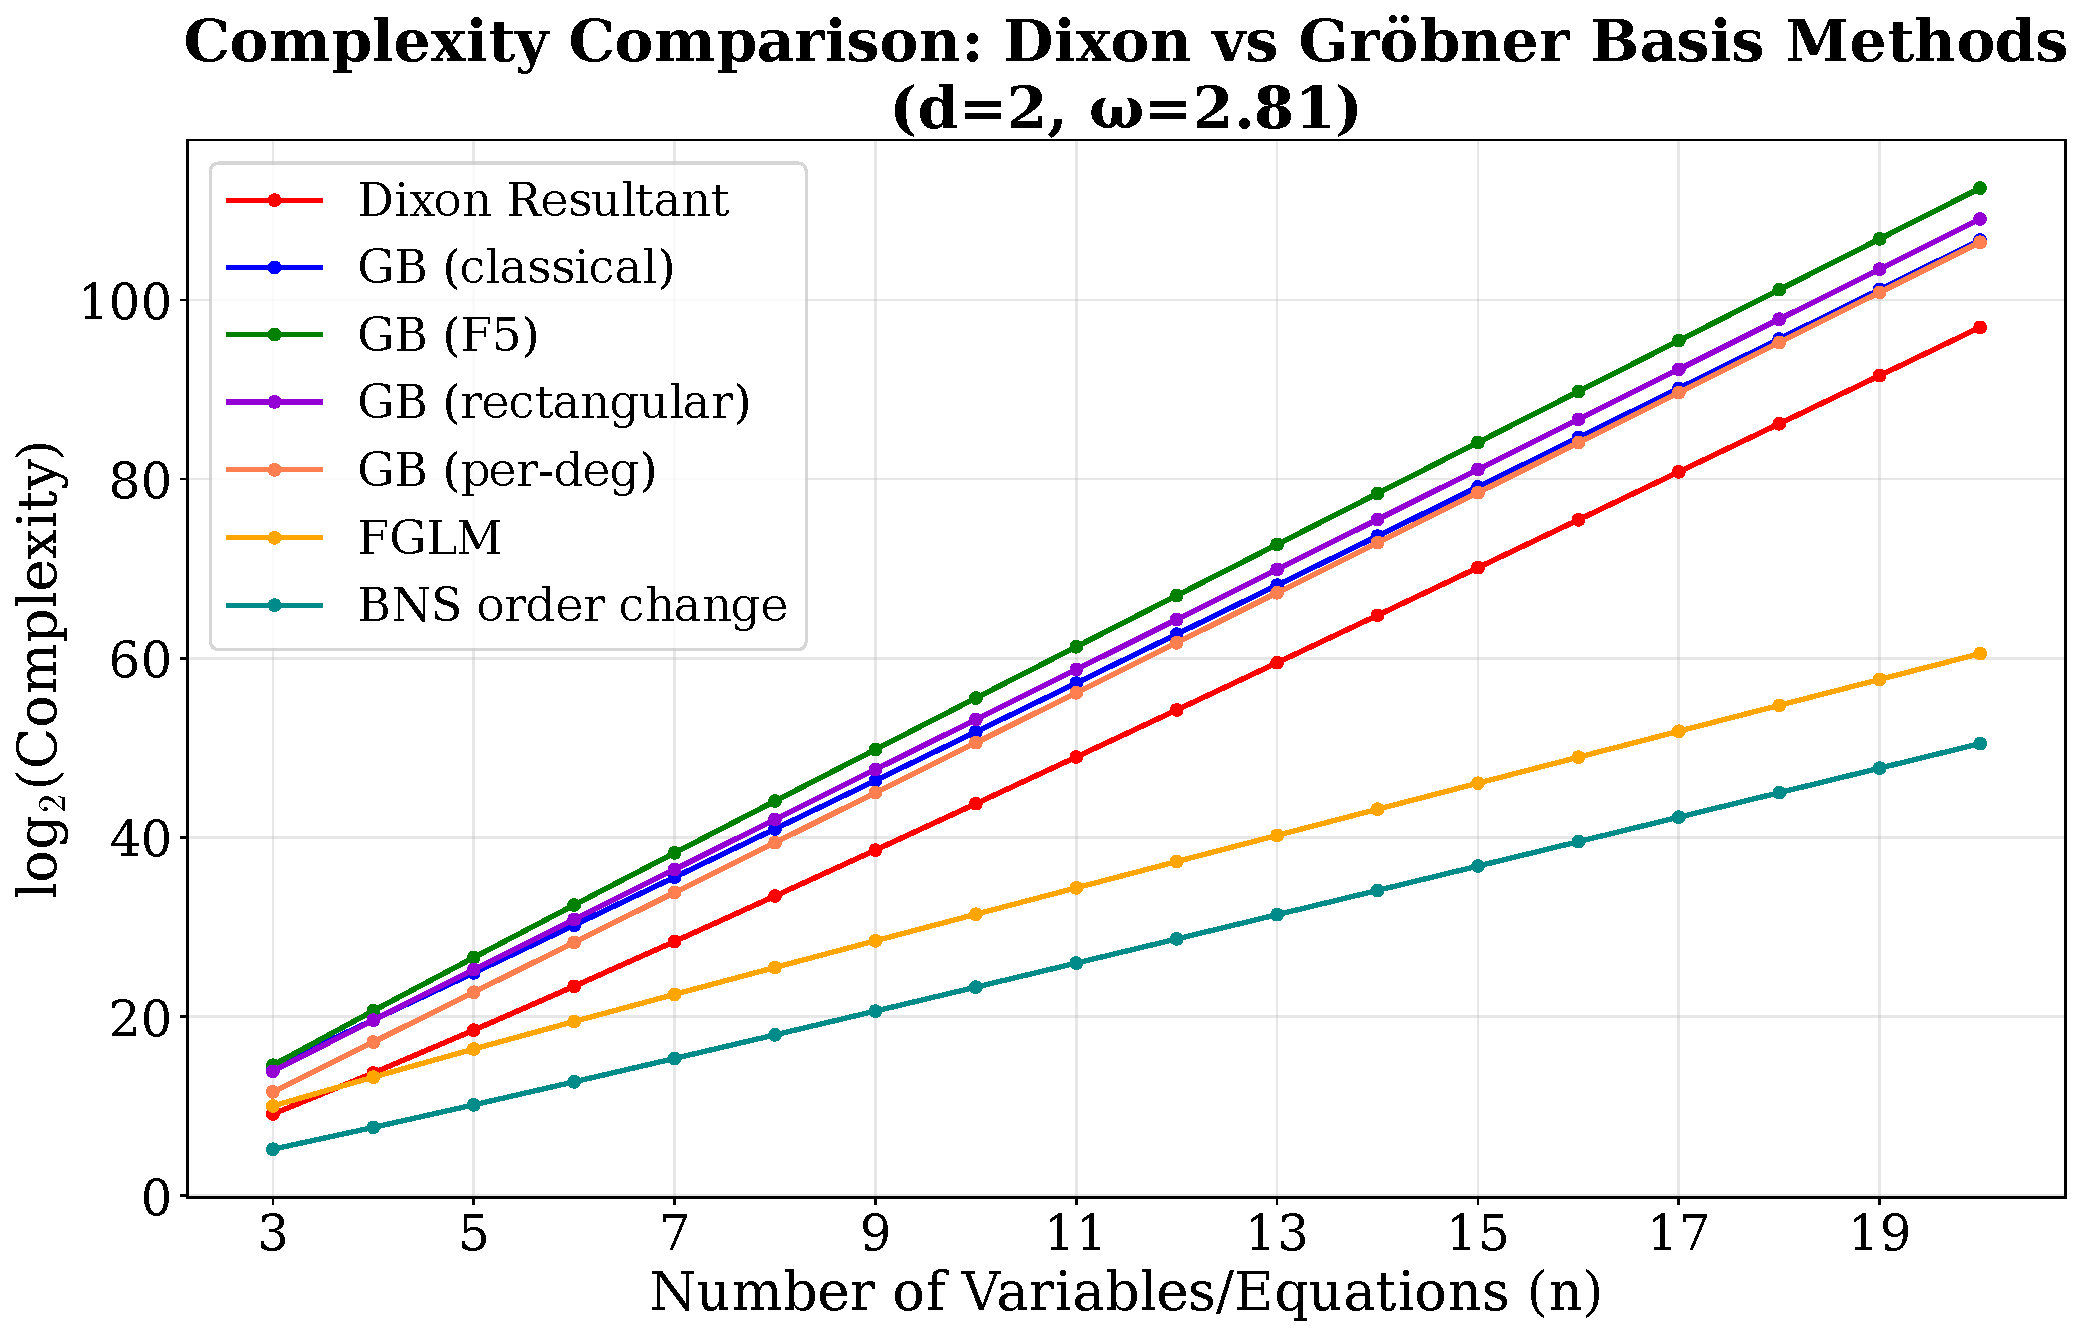
\includegraphics[width=0.99\textwidth]{complexity_comparison_d2.pdf}
	\caption{Complexity comparison varying $n$ with $d=2$, $\omega=2.81$. }
	\label{fig:complexity_comparison_d}
\end{figure}


\subsubsection{Overdetermined Systems ($m > n$)}

Gr\"obner basis methods are typically preferable here: the degree of regularity is significantly lower than for well-determined systems~\cite{Faugere2004}, and the grevlex basis often yields univariate polynomials directly, eliminating the FGLM step. The Dixon resultant, in contrast, needs exactly $n$ equations to eliminate $n-1$ variables and cannot leverage redundancy: one selects $n$ equations and verifies the rest afterward, at slightly higher cost than the well-determined case.

\subsubsection{Underdetermined Systems ($m < n$)}

For complete solving, a common cryptanalytic strategy is to guess $n-m$ variables and solve the resulting subsystem using Gr\"obner bases; we do not propose Dixon as a replacement. For elimination in this positive-dimensional setting, however, Dixon treats the retained variables as parameters and eliminates several variables at once, producing explicit relations that can be combined with guessing or meet-in-the-middle decompositions; by contrast, Gr\"obner-basis conversion in the same setting
may use Gr\"obner walks~\cite{DBLP:journals/jsc/CollartKM97}, whose cost can be difficult to predict.

\smallskip\noindent
In summary, the two methods are complementary: Dixon and Gr\"obner basis are comparable on well-determined systems; Gr\"obner basis is typically preferable for overdetermined systems; Dixon is attractive for underdetermined systems as a determinant-based elimination method.
